%\documentclass[handout]{beamer}
\documentclass{beamer}
\usepackage[ruled,linesnumbered]{algorithm2e}
\usepackage{natbib}
%\usepackage{enumitem}
\definecolor{vuborange}{rgb}{1.0,0.40,0.0}
\usetheme{Boadilla}
\usepackage{amsmath,amssymb}
\usepackage{booktabs}
\title{Efficiently Explaining CSPs with Unsatisfiable Subset Optimization}
\institute[shortinst]
{\inst{1} Vrije Universiteit Brussel, Belgium \\ % Your institution for the title page
	\inst{2} KULeuven, Belgium \\ % Your institution for the title page
	\href{mailto:emilio.gamba@vub.be}{\underline{emilio.gamba@vub.be}}, \href{mailto:bart.bogaerts@vub.be}{bart.bogaerts@vub.be}, \href{mailto:tias.guns@kuleuven.be}{tias.guns@kuleuven.be} % Your email address
}
\date{IJCAI 2021}

\author{\underline{Emilio Gamba}\inst{1} \and  Bart Bogaerts\inst{1} \and   Tias Guns\inst{1,2}}

\newcommand\m[1]{\ensuremath{#1}\xspace}
\newcommand\allconstraints{\m{T_P}}
\newcommand\formula{\ensuremath{\m{F} }\xspace}
\newcommand\formulac{\ensuremath{\m{C} }\xspace}

\makeatletter
\setbeamertemplate{footline}
{
	\leavevmode%
	\hbox{%
		\begin{beamercolorbox}[wd=.2\paperwidth,ht=2.25ex,dp=1ex,center]{author in head/foot}%
			\usebeamerfont{author in head/foot}Emilio Gamba (VUB)
		\end{beamercolorbox}%
		\begin{beamercolorbox}[wd=.6\paperwidth,ht=2.25ex,dp=1ex,center]{title in head/foot}%
			\usebeamerfont{title in head/foot}Efficiently Explaining CSPs with Unsatisfiable Subset Optimization
		\end{beamercolorbox}%
		\begin{beamercolorbox}[wd=.2\paperwidth,ht=2.25ex,dp=1ex,right]{date in head/foot}%
			\usebeamerfont{date in head/foot}August 2021\hspace*{1em}
			\insertframenumber{} / \inserttotalframenumber\hspace*{2ex} 
	\end{beamercolorbox}}%
	\vskip0pt%
}
\makeatother

\begin{document}
%	We build on a recently proposed method for explaining solutions of constraint satisfaction problems.
%	An explanation here is a \textit{sequence} of simple inference steps, where the simplicity of an inference step is measured by the number and types of constraints and facts used, and where the sequence explains all logical consequences of the problem. 
%	We build on these formal foundations and tackle two emerging questions, namely how to generate explanations that are provably optimal (with respect to the given cost metric) and how to generate them efficiently. 
%	To answer these questions, we develop 1) an implicit hitting set algorithm for finding \textit{optimal} unsatisfiable subsets; 2) a method to reduce multiple calls for (optimal) unsatisfiable subsets to a single call that takes \emph{constraints} on the subset into account, and 3) a method for re-using relevant information over multiple calls to these algorithms. 
%	The method is also applicable to other problems that require finding cost-optimal unsatisfiable subsets.
%	We specifically show that this approach can be used to effectively find sequences of \textit{optimal} explanation steps for constraint satisfaction problems like logic grid puzzles.
	\begin{frame}
		\maketitle
	\end{frame}
	
	
	\begin{frame}{Motivation}
		\framesubtitle{Step-wise Explanations of CSPs}
		\cite{bogaerts2020step} proposed a method for explaining solutions of constraint satisfaction problems.\pause
		
		\begin{definition}
			An \emph{\color{vuborange}explanation} is defined as a \textit{sequence} of simple inference steps. 
		\end{definition}\pause

		\begin{definition}
			\emph{\color{vuborange}Simplicity} of an explanation is measured by the number and types of constraints and facts used.
		\end{definition}
	\end{frame}
		
	\begin{frame}{Motivation}
		\framesubtitle{Open questions}
		\begin{description}[font=\color{vuborange}\itshape]
			\item[Optimality] Explanations not optimal, \emph{heuristically} found \pause
			\item[Efficiency] Explanation generation takes a lot of time \pause
			\item[Incrementality] Can we \emph{reuse information} from an explanation call to another? \pause
			\item[Constrainedness] Can we \emph{avoid looping over the literals} when searching for the next best explanation ?
		\end{description}
	\end{frame}
	
%	\begin{itemize}
%		\item[$\rightsquigarrow$] \emph{\color{vuborange} Cost function} as a proxy for explanation difficulty.
%	\end{itemize}
%
%%	\begin{frame}{Contributions}
%%		We introduce a method for finding \emph{\color{vuborange}cost-optimal} unsatisfiable subsets (\emph{\color{vuborange}OUS}). \pause
%%		\begin{description}[font=\color{vuborange}\itshape]
%%			\item[Optimality] 
%%%			\emph{\color{vuborange} Cost function} as a proxy for explanation difficulty.
%%%			\item[Efficiency]\emph{\color{vuborange} Implicit hitting set algorithm.}
%%%			\item[Incrementality]  \emph{\color{vuborange} Information reuse} over multiple similar calls
%%%			\item[Constrainedness]  Add constraints on the \emph{\color{vuborange}shape of explanation} to the implicit hitting set algorithm.
%%
%%		\end{description}
%%	\end{frame}
%
%	\begin{frame}{Contributions}
%	We introduce a method for finding \emph{\color{vuborange}cost-optimal} unsatisfiable subsets (\emph{\color{vuborange}OUS}).
%	\begin{description}[font=\color{vuborange}\itshape]
%		\item[Optimality] \emph{\color{vuborange} Cost function} as a proxy for explanation difficulty.
%%		\item[Efficiency]\emph{\color{vuborange} Implicit hitting set algorithm.}
%%		\item[Incrementality]  \emph{\color{vuborange} Information reuse} over multiple similar calls
%%		\item[Constrainedness]  Add constraints on the \emph{\color{vuborange}shape of explanation} to the implicit hitting set algorithm.
%%		
%	\end{description}
%\end{frame}
%
%%	\begin{frame}{Contributions}
%%	We introduce a method for finding \emph{\color{vuborange}cost-optimal} unsatisfiable subsets (\emph{\color{vuborange}OUS}).
%%	\begin{description}[font=\color{vuborange}\itshape]
%%		\item[Optimality] \emph{\color{vuborange} Cost function} as a proxy for explanation difficulty.
%%		\item[Efficiency]
%%%		\emph{\color{vuborange} Implicit hitting set algorithm.}
%%%		\item[Incrementality]  \emph{\color{vuborange} Information reuse} over multiple similar calls
%%%		\item[Constrainedness]  Add constraints on the \emph{\color{vuborange}shape of explanation} to the implicit hitting set algorithm.
%%%		
%%	\end{description}
%%\end{frame}
%
%	\begin{frame}{Contributions}
%	We introduce a method for finding \emph{\color{vuborange}cost-optimal} unsatisfiable subsets (\emph{\color{vuborange}OUS}).
%	\begin{description}[font=\color{vuborange}\itshape]
%		\item[Optimality] \emph{\color{vuborange} Cost function} as a proxy for explanation difficulty.
%		\item[Efficiency]\emph{\color{vuborange} Implicit hitting set algorithm.}
%%		\item[Incrementality]  \emph{\color{vuborange} Information reuse} over multiple similar calls
%%		\item[Constrainedness]  Add constraints on the \emph{\color{vuborange}shape of explanation} to the implicit hitting set algorithm.
%%		
%	\end{description}
%\end{frame}
%
%%	\begin{frame}{Contributions}
%%	We introduce a method for finding \emph{\color{vuborange}cost-optimal} unsatisfiable subsets (\emph{\color{vuborange}OUS}).
%%	\begin{description}[font=\color{vuborange}\itshape]
%%		\item[Optimality] \emph{\color{vuborange} Cost function} as a proxy for explanation difficulty.
%%		\item[Efficiency]\emph{\color{vuborange} Implicit hitting set algorithm.}
%%		\item[Incrementality] 
%%%		 \emph{\color{vuborange} Information reuse} over multiple similar calls
%%%		\item[Constrainedness]  Add constraints on the \emph{\color{vuborange}shape of explanation} to the implicit hitting set algorithm.
%%		
%%	\end{description}
%%\end{frame}
%
%	\begin{frame}{Contributions}
%	We introduce a method for finding \emph{\color{vuborange}cost-optimal} unsatisfiable subsets (\emph{\color{vuborange}OUS}).
%	\begin{description}[font=\color{vuborange}\itshape]
%		\item[Optimality] \emph{\color{vuborange} Cost function} as a proxy for explanation difficulty.
%		\item[Efficiency]\emph{\color{vuborange} Implicit hitting set algorithm.}
%		\item[Incrementality]  \emph{\color{vuborange} Information reuse} over multiple similar calls
%%		\item[Constrainedness]  Add constraints on the \emph{\color{vuborange}shape of explanation} to the implicit hitting set algorithm.
%%		
%	\end{description}
%\end{frame}
%
%%	\begin{frame}{Contributions}
%%	We introduce a method for finding \emph{\color{vuborange}cost-optimal} unsatisfiable subsets (\emph{\color{vuborange}OUS}). 
%%	\begin{description}[font=\color{vuborange}\itshape]
%%		\item[Optimality] \emph{\color{vuborange} Cost function} as a proxy for explanation difficulty.
%%		\item[Efficiency]\emph{\color{vuborange} Implicit hitting set algorithm.}
%%		\item[Incrementality]  \emph{\color{vuborange} Information reuse} over multiple similar calls
%%		\item[Constrainedness] 
%%%		 Add constraints on the \emph{\color{vuborange}shape of explanation} to the implicit hitting set algorithm.
%%	\end{description}
%%\end{frame}


%			\item[Optimality] Explanations not optimal, heuristically found \pause
%\item[Efficiency] Explanation generation takes a lot of time \pause
%\item[Incrementality] Can we reuse information from an explanation call to another? \pause
%\item[Constrainedness] Can we avoid looping over the literals when searching for the next best explanation ?

%	\begin{frame}{Contributions}
%	We introduce a method for finding \emph{\color{vuborange}cost-optimal} unsatisfiable subsets (\emph{\color{vuborange}OUS}).
%	\begin{description}[font=\color{vuborange}\itshape]
%		\item[Optimality] Explanations not optimal, heuristically found.
%			\begin{itemize}
%			\item[$\rightsquigarrow$] \emph{\color{vuborange} Cost function} as a proxy for explanation difficulty.
%		\end{itemize} \pause
%		\item[Efficiency] Explanation generation takes a lot of time
%					\begin{itemize}
%			\item[$\rightsquigarrow$] \emph{\color{vuborange} Implicit hitting set algorithm.}
%		\end{itemize} \pause
%		\item[Incrementality]  Can we reuse information from an explanation call to another?
%					\begin{itemize}
%			\item[$\rightsquigarrow$]\emph{\color{vuborange} Information reuse} over multiple similar calls
%		\end{itemize} \pause
%		\item[Constrainedness]  Can we avoid looping over the literals when searching for the next best explanation ?
%					\begin{itemize}
%			\item[$\rightsquigarrow$] Add \emph{\color{purple}constraints} on the \emph{\color{vuborange}shape of explanation} to the implicit hitting set algorithm.
%		\end{itemize} 
%	\end{description}
%\end{frame}

	\begin{frame}{Contributions}
	We introduce a method for finding \emph{\color{vuborange}cost-optimal constrained} unsatisfiable subsets (\emph{\color{vuborange}OCUS}), where
	\begin{description}[font=\color{vuborange}\itshape]
		\onslide<1->{\item[Optimality] \emph{\color{vuborange} Cost function} is a proxy for explanation difficulty.}
	\onslide<2->{\item[Efficiency]\emph{\color{vuborange} Implicit hitting set algorithm} based on the hitting set duality of \cite{ignatiev2015smallest}.}
		\end{description}
	\only<2>{	
		\begin{figure}
			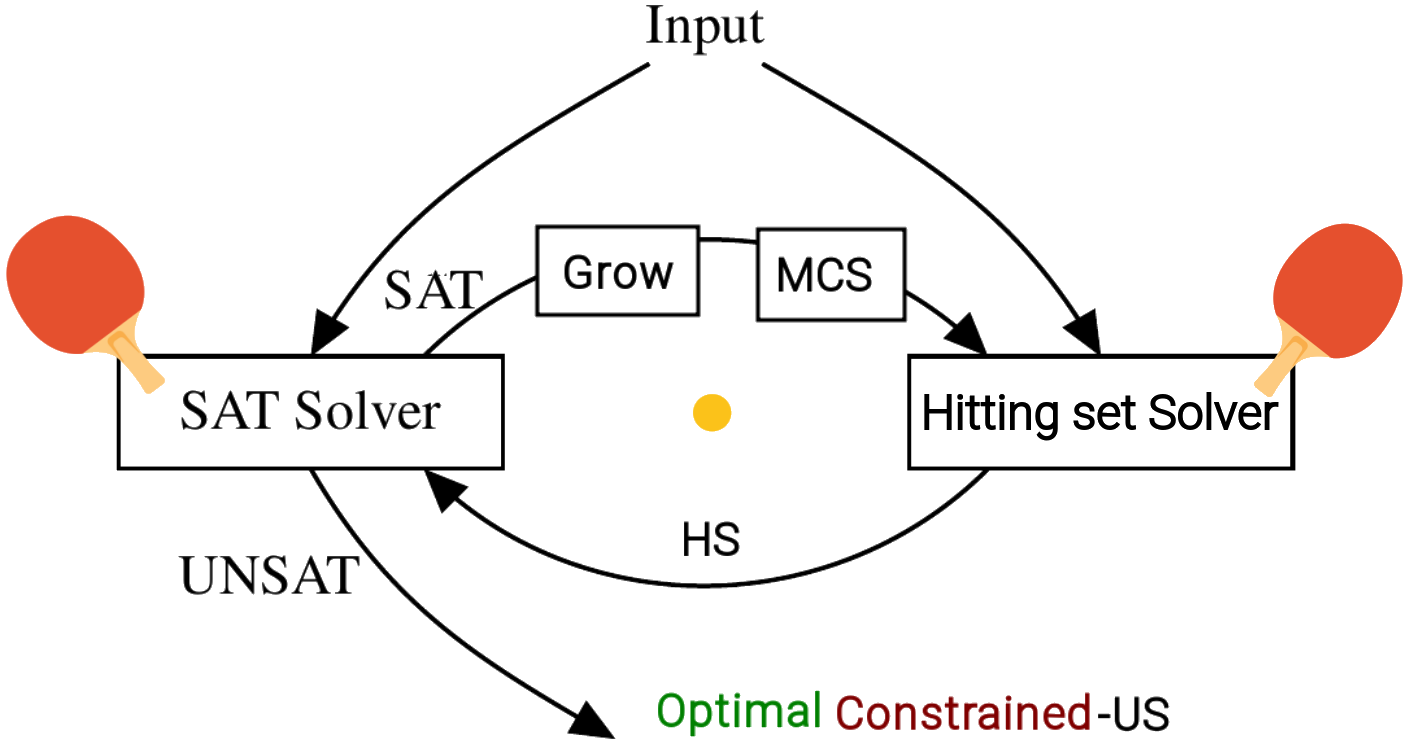
\includegraphics[width=0.7\linewidth]{ihs_constrained.png}
			\caption{Implicit hitting set algorithm\footnote{Figure inspired by \cite{saikko2016implicit}}}
		\end{figure}
	}
		\begin{description}[font=\color{vuborange}\itshape]
	\onslide<3->{\item[Incrementality]  \emph{\color{vuborange} Information reuse} over multiple similar calls.}
	\onslide<4->{\item[Constrainedness]  Add \emph{\color{purple}constraints} on the \emph{\color{vuborange}shape of explanation} to the implicit hitting set algorithm.}
	\end{description}
	\only<1>{	
	\vspace{5cm}}
	\onslide<3->{	
\begin{figure}
	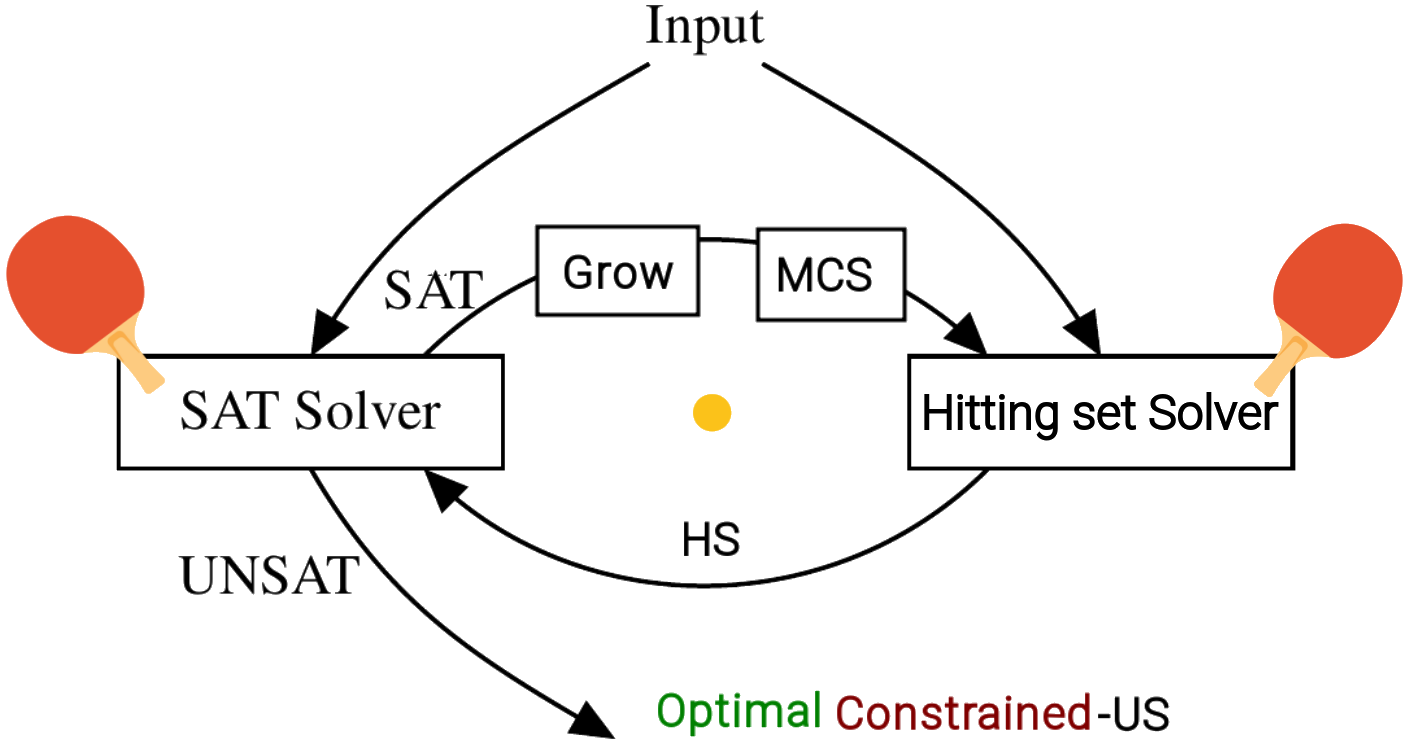
\includegraphics[width=0.35\linewidth]{ihs_constrained.png}
	\caption{Implicit hitting set algorithm\footnote{Figure inspired by \cite{saikko2016implicit}}}
\end{figure}
}
\end{frame}
%
%	\begin{frame}{Contributions}
%	We introduce a method for finding \emph{\color{vuborange}cost-optimal} unsatisfiable subsets (\emph{\color{vuborange}OUS}).
%	\begin{description}[font=\color{vuborange}\itshape]
%		\item[Optimality] \emph{\color{vuborange} Cost function} as a proxy for explanation difficulty.
%		\item[Efficiency]\emph{\color{vuborange} Implicit hitting set algorithm.}
%		\item[Incrementality]  \emph{\color{vuborange} Information reuse} over multiple similar calls\pause
%		\item[Constrainedness]  Add \emph{\color{purple}constraints} on the \emph{\color{vuborange}shape of explanation} to the implicit hitting set algorithm.
%	\end{description}
%\end{frame}

%
%	\begin{frame}{Open questions and Contributions}
%	We introduce a method for finding cost-optimal unsatisfiable subsets (OUS).
%	\begin{description}[font=\color{vuborange}\itshape]
%		\item[Optimality] \pause \emph{\color{vuborange} Cost function} as a proxy for explanation difficulty.\pause
%		\item[Efficiency] \pause \emph{\color{vuborange} Implicit hitting set algorithm.}\pause
%		\item[Incrementality] \pause \emph{\color{vuborange} Information reuse} over multiple similar calls\pause
%		\item[Constrainedness] \pause  Add constraints on the \emph{\color{vuborange}shape of explanation} to the implicit hitting set algorithm.\pause
%
%	\end{description}
	
%\end{frame}


%		\begin{figure}
%			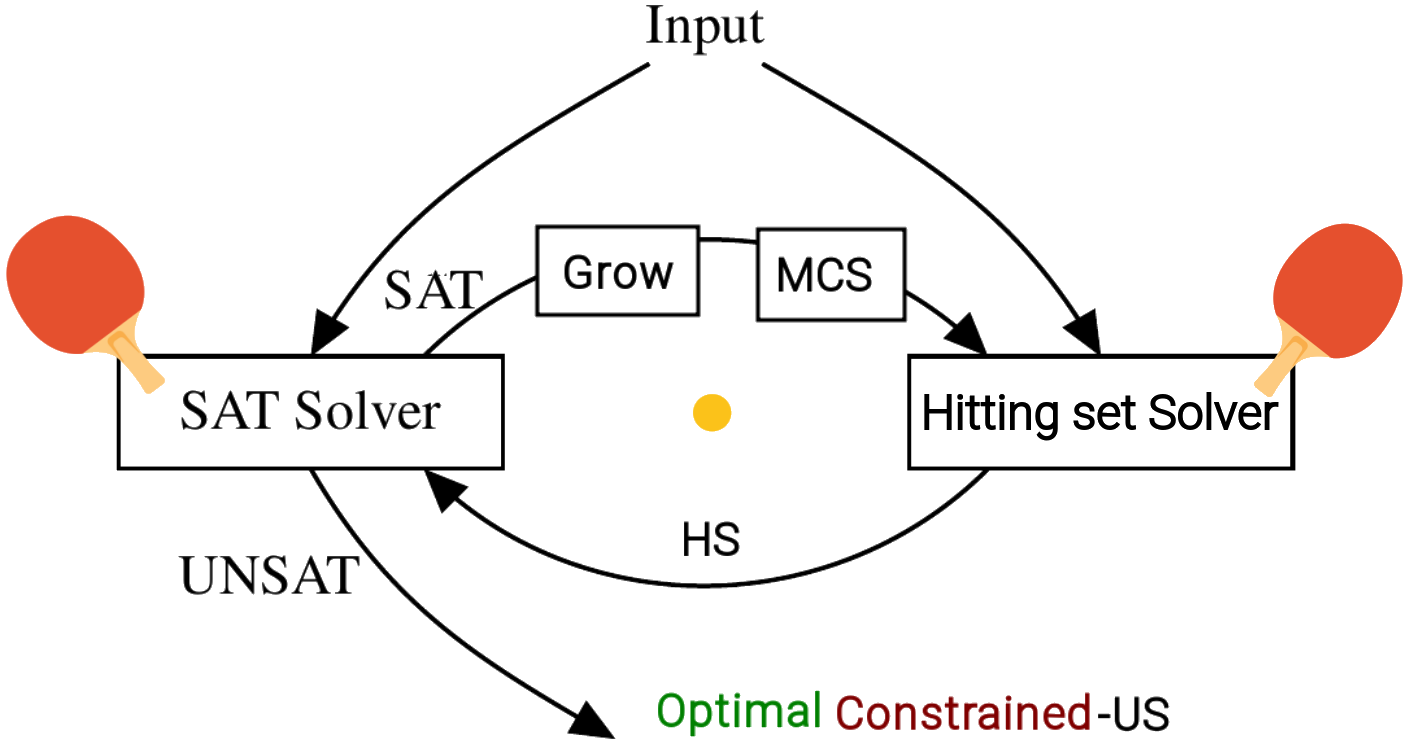
\includegraphics[width=0.4\textwidth]{ihs_constrained.png}
%			\caption{Implicit hitting set algorithm}
%		\end{figure}
%	\begin{frame}
%	\begin{description}[font=\color{vuborange}\itshape]
%		\item[Optimality] Explanations not optimal, heuristically found \pause
%		\begin{itemize}
%			\item \emph{\color{vuborange} Cost function as a proxy for explanation difficulty.}
%		\end{itemize}
%		\item[Efficiency] Explanation generation takes a lot of time \pause
%		\begin{itemize}
%			\item \emph{\color{vuborange} Implicit hitting set algorithm.}
%			\item \emph{\color{vuborange} Single call to find optimal explanation}
%		\end{itemize}
%		\item[Constrainedness] Can we avoid looping over the literals when searching for the next best explanation ?
%		\begin{itemize}
%			\item \emph{\color{vuborange} Add constraint to the Implicit hitting set algorithm.}
%		\end{itemize}
%		\item[Incrementality] Can we reuse information from an explanation call to another? \pause
%		\begin{itemize}
%			\item \emph{\color{vuborange} Information reuse over multiple similar calls}
%		\end{itemize}
%	\end{description}
%	\begin{description}
%		\item[Optimality] Cost function as a proxy for explanation difficulty
%		\item[Efficiency] Single optimal explanation
%		\item[Constrainedness] Implicit hitting set algorithm.
%		\item[Incrementality] Information reuse over multiple similar calls.
%	\end{description}
%\end{minipage}
%		\begin{description}[font=\color{vuborange}\itshape]
%			\item[\hspace{0.9cm}Optimality] Explanations not optimal, heuristically found \pause
%			\item[\hspace{1.05cm}Efficiency] Explanation generation takes a lot of time \pause
%			\item[\hspace{0.3cm}Incrementality] Can we reuse information from an explanation call to another? \pause
%			\item[Constrainedness] Can we avoid looping over the literals when searching for the next best explanation ?
%		\end{description}
%	\end{frame}
%	\begin{frame}
%		\frametitle{Outline}
%		
%		\begin{enumerate}
%			\item Motivation
%			\begin{itemize}
%				\item Explanations for logic puzzles (but also for CSPs)
%				\item Generating an explanation sequence for CSPs
%			\end{itemize}
%			\item Contributions and Applicability
%			\begin{enumerate}
%				\item Optimality \& Constrainedness
%				\item Incrementality
%			\end{enumerate}
%			\item Results
%			\item Conclusion
%			\item Ideas for future work
%		\end{enumerate}
%	\end{frame}
%	
%	\begin{frame}{Motivation}
%		\framesubtitle{Logic Grid Puzzles}
%		\begin{figure}
%			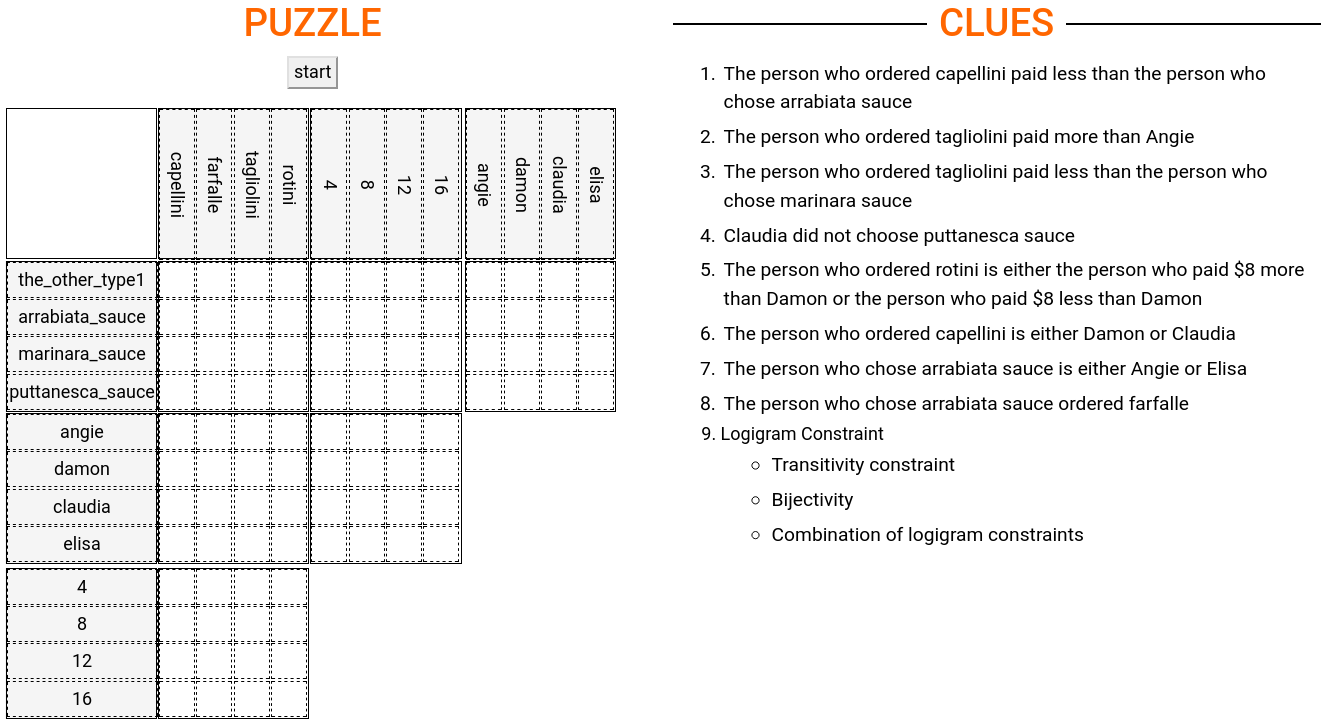
\includegraphics[width=0.9\textwidth]{logicpuzzles.png}
%		\end{figure}
%		\begin{center}
%			\url{https://bartbog.github.io/zebra/pasta/}
%		\end{center}
%	\end{frame}
%	
%	\begin{frame}{Motivation}
%		\framesubtitle{CSPs: a little formal Background}
%		
%		\begin{itemize}
%			%               \setlength{\leftmargin}{0pt}
%			\item[$\m{C}$] \emph{constraints} we can use to reason (alldifferent, George did not take pasta, …)
%			\item[$\mathcal{I}_0$] an \emph{Initial Interpretation}
%			\item[$\mathcal{I}_{end}$] Everything we can derive from $ \m{C} \wedge \mathcal{I}_0$
%		\end{itemize}
%		\begin{figure}
%			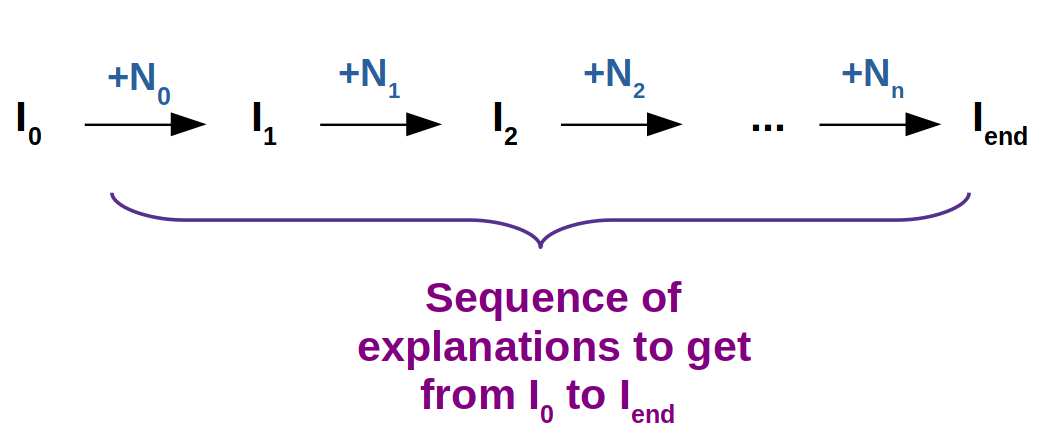
\includegraphics[width=0.7\textwidth]{sequence_explanation.png}
%		\end{figure}
%	\end{frame}
%	
%	
%	\begin{frame}{Motivation}
%		\framesubtitle{Gentle reminder: Explanations for CSPs}
%		\begin{definition}
%			Given one or a subset of the constraints ( $S_i \subseteq T_P$  ) and facts we know ($E_i\subseteq \mathcal{I}_i$), an \textbf{explanation} is an implication of the form $E_i \wedge S_i  \implies N_i $, where $N_i$ is the new information from $S_i \cup E_i \models N_i$. \cite{bogaerts2020step}
%		\end{definition}
%		
%	\end{frame}
%	
%	\begin{frame}{Motivation}
%		\begin{figure}
%			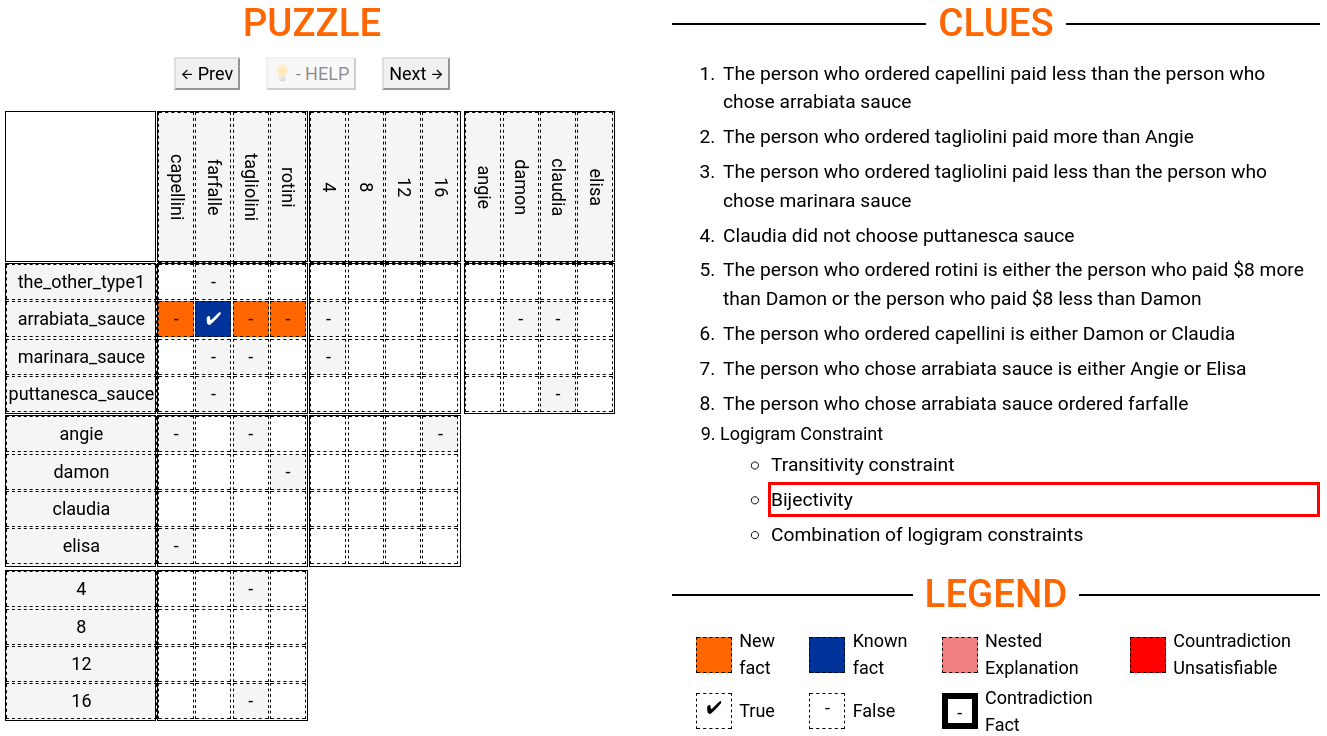
\includegraphics[width=0.8\textwidth]{logic_puzzles_bij.png}
%		\end{figure}\pause
%		\begin{itemize}
%			\item[$E_i$] farfalle goes with arrabiata sauce \pause
%			\item[$S_i$] an entity of type pasta can only be linked to one entity of type sauce\pause
%			\item[$N_i$] taglioni, rotini and capellini cannot be linked to arriabiata
%		\end{itemize}
%		
%	\end{frame}
%	
%	\newcommand\onestep{\ensuremath{\call{explain-One-Step}}\xspace}
%	
%		\begin{frame}{Motivation}
%		\framesubtitle{Gentle reminder: Explanations for CSPs}
%		\begin{definition}
%			Given one or a subset of the constraints ( $S_i \subseteq T_P$  ) and facts we know ($E_i\subseteq \mathcal{I}_i$), an \textbf{explanation} is an implication of the form $E_i \wedge S_i  \implies N_i $, where $N_i$ is the new information from $S_i \cup E_i \models N_i$. \cite{bogaerts2020step}
%		\end{definition} 
%		
%		An \textbf{explanation sequence} is of the form $$<(\mathcal{I}_0,(\emptyset,\emptyset,\emptyset)),\text{\hspace{3pt}}(\mathcal{I}_1,(E_1, S_1, N_1)),\text{\hspace{3pt}}...,\text{\hspace{3pt}}(\mathcal{I}_{end},(E_{n}, S_n, N_n ))>$$
%		
%		\begin{figure}
%			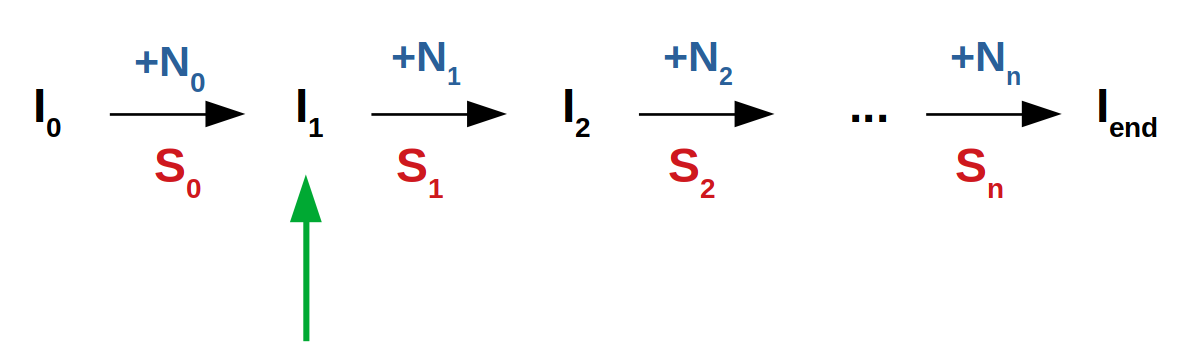
\includegraphics[width=0.7\textwidth]{sequence_explanation2.png}
%		\end{figure}
%		
%	\end{frame}
%	
%	\begin{frame}{Motivation}
%		\framesubtitle{Generating an explanation sequence for CSPs}
%\cite{bogaerts2020step}: At every step in the explanation sequence:
%		\begin{figure}
%			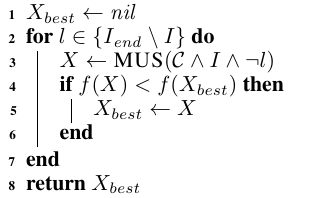
\includegraphics[width=0.45\textwidth]{algo_mus2.png}
%		\end{figure}
%		\begin{itemize}
%			\item Finding non-redundant explanations: MUS($\formulac \land \mathcal{I} \land \neg l$) extraction (IDP system)
%			
%		\end{itemize}
%	\end{frame}
%
%	\begin{frame}{Motivation}
%	\framesubtitle{Generating an explanation sequence for CSPs}
%\cite{bogaerts2020step}: At every step in the explanation sequence:
%	\begin{figure}
%		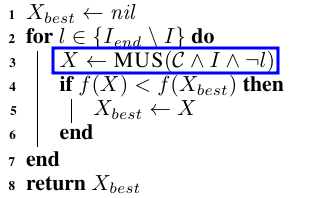
\includegraphics[width=0.45\textwidth]{algo_mus2_b.png}
%	\end{figure}
%	\begin{itemize}
%		\item Finding non-redundant explanations: MUS($\formulac \land \mathcal{I} \land \neg l $) extraction (IDP system)
%		
%		\begin{itemize}
%			\item In practice, not all constraints at once!
%			\item Consider power sets of constraints sorted by increasing cost
%		\end{itemize}
%	\end{itemize}
%\end{frame}
%
%	
%	\begin{frame}{Motivation}
%		\framesubtitle{Open Questions}
%		
%		\begin{description}[font=\color{vuborange}\itshape]
%			\item[\hspace{0.9cm}Optimality] Explanations not optimal, heuristically found \pause
%			\item[\hspace{1.05cm}Efficiency] Explanation generation takes a lot of time \pause
%			\item[\hspace{0.3cm}Incrementality] Can we reuse information from an explanation call to another? \pause
%			\item[Constrainedness] Can we avoid looping over the literals when searching for the next best explanation ?
%		\end{description}
%	\end{frame}
%	
%	\begin{frame}{Optimality}
%		\pause
%		\begin{minipage}{0.49\textwidth}
%						\begin{figure}
%				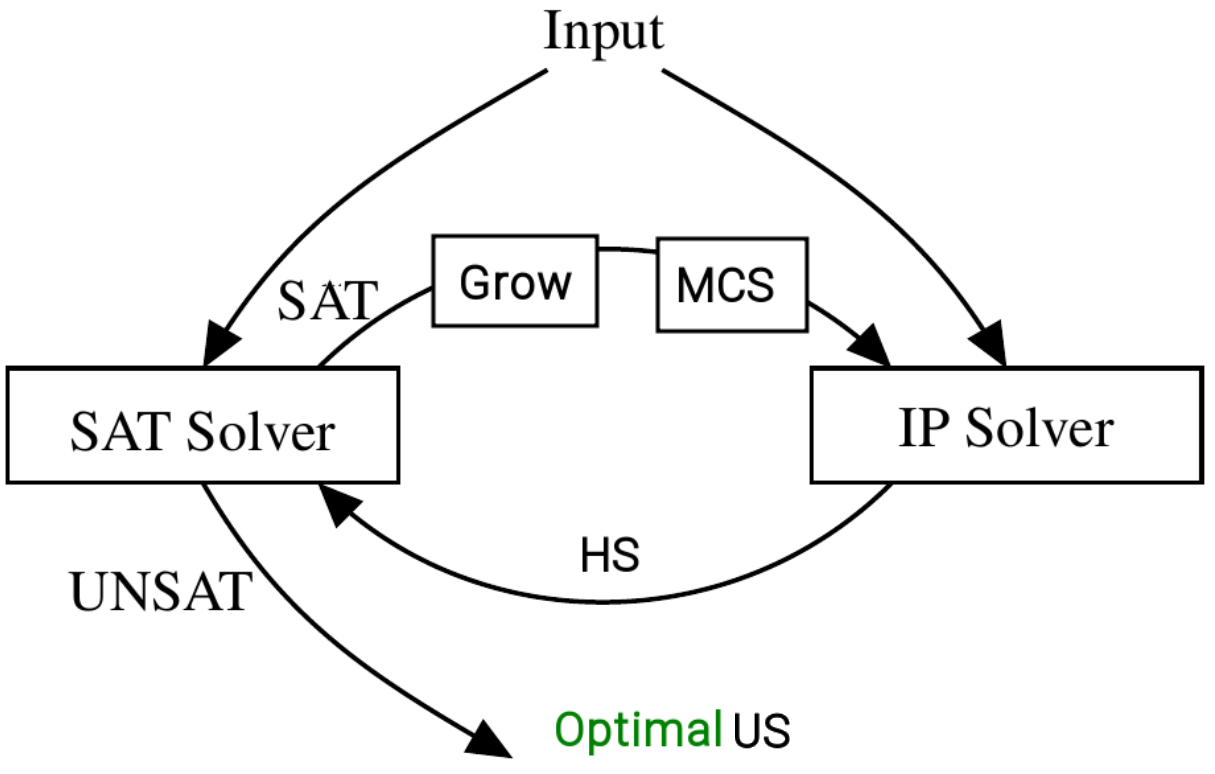
\includegraphics[width=\textwidth]{ihs.png}
%			\end{figure}
%			\pause
%		\end{minipage}
%		\begin{minipage}{0.5\textwidth}
%		\begin{itemize}
%			\item Inspired by \cite{ignatiev2015smallest}
%			\item MIP solver instead of SAT-based
%			\item[+] Optimal Hitting set (\emph{\textbf{Optimality}})
%		\end{itemize}
%		\end{minipage}
%		\vfill
%		\begin{figure}
%			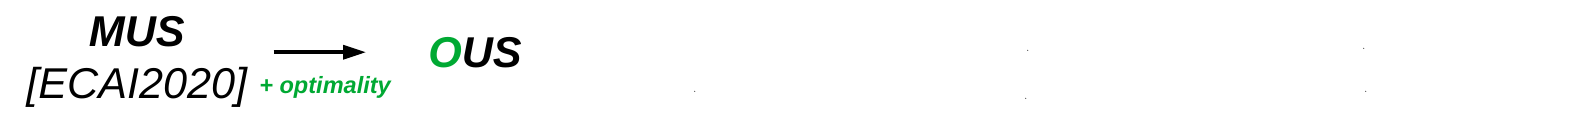
\includegraphics[width=\textwidth]{mus_to_ous.png}
%		\end{figure}
%		
%	\end{frame}
%
%\begin{frame}{Optimality}
%	\framesubtitle{Verifying explanation quality}
%	\pause
%			\begin{figure}
%		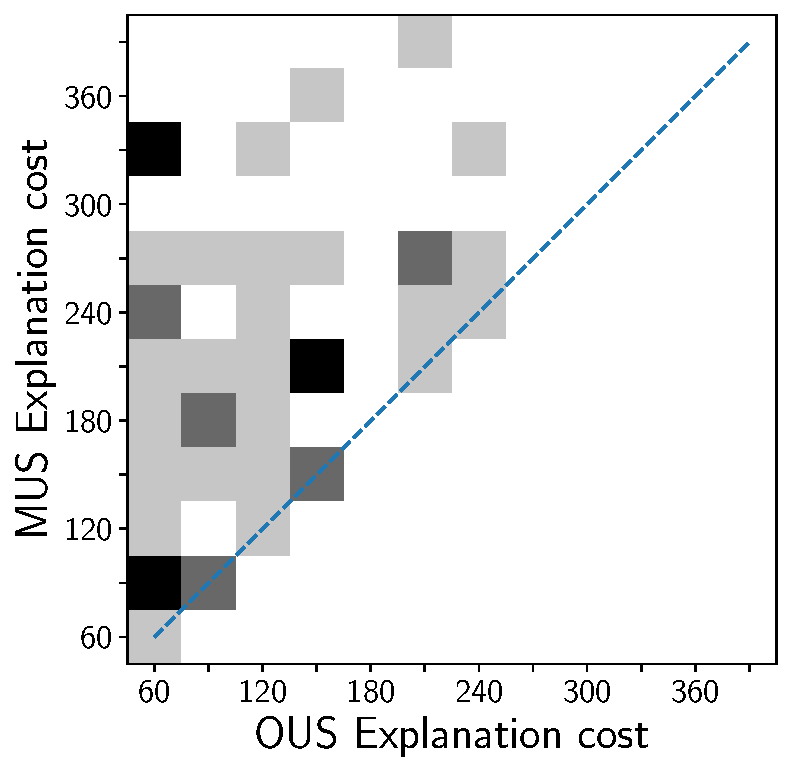
\includegraphics[width=0.6\textwidth]{heatmap_costs_mus_cous.pdf}
%	\end{figure}
%\end{frame}
%	
%	
%	
%	
%		\begin{frame}{Incrementality}
%			\framesubtitle{Improving efficiency of OUS}
%		
%		\begin{minipage}{0.59\textwidth}
%			\begin{enumerate}
%				\item {\color{vuborange} Incremental \emph{OUSs} }
%				\begin{itemize}
%					\item Keep Satisfiable Subsets between OUS-calls
%				\end{itemize}	
%			\end{enumerate}
%		\end{minipage}
%		\begin{minipage}{0.4\textwidth}
%			\begin{figure}
%				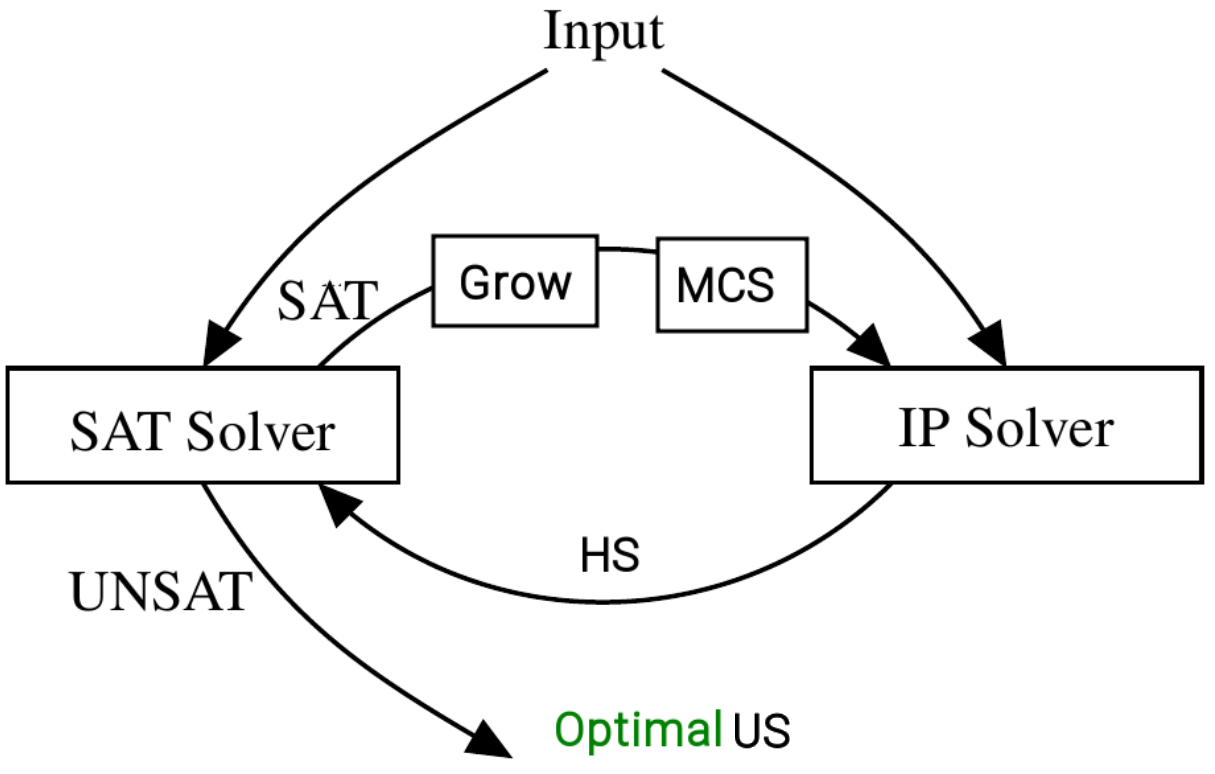
\includegraphics[width=\textwidth]{ihs.png}
%			\end{figure}
%		\end{minipage}
%		\vfill
%		\begin{figure}
%			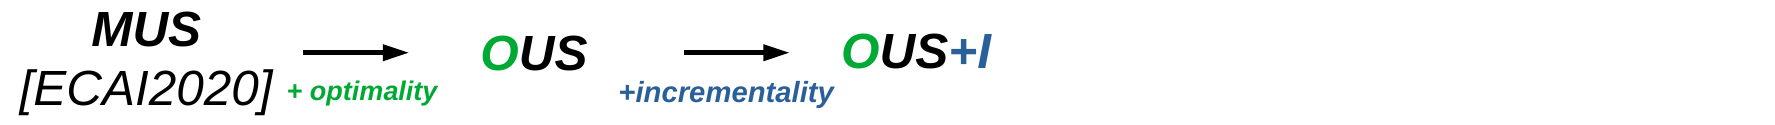
\includegraphics[width=\textwidth]{mus_to_ous_i.png}
%		\end{figure}
%	\end{frame}
%	
%	
%	
%	\begin{frame}{Incrementality}
%		
%		\begin{minipage}{0.59\textwidth}
%			\begin{enumerate}
%				\item {\color{vuborange} Incremental \emph{OUSs} }
%				\begin{itemize}
%					\item Keep Satisfiable Subsets between OUS-calls
%					\item Naïve OUS-restart $\rightarrow$ Keep 1 MIP solver warm per literal
%					\begin{itemize}
%						\item[$\implies$] No need to keep track of Satisfiable Subsets
%					\end{itemize}
%				\end{itemize}	
%			\end{enumerate}
%		\end{minipage}
%		\begin{minipage}{0.4\textwidth}
%			\begin{figure}
%				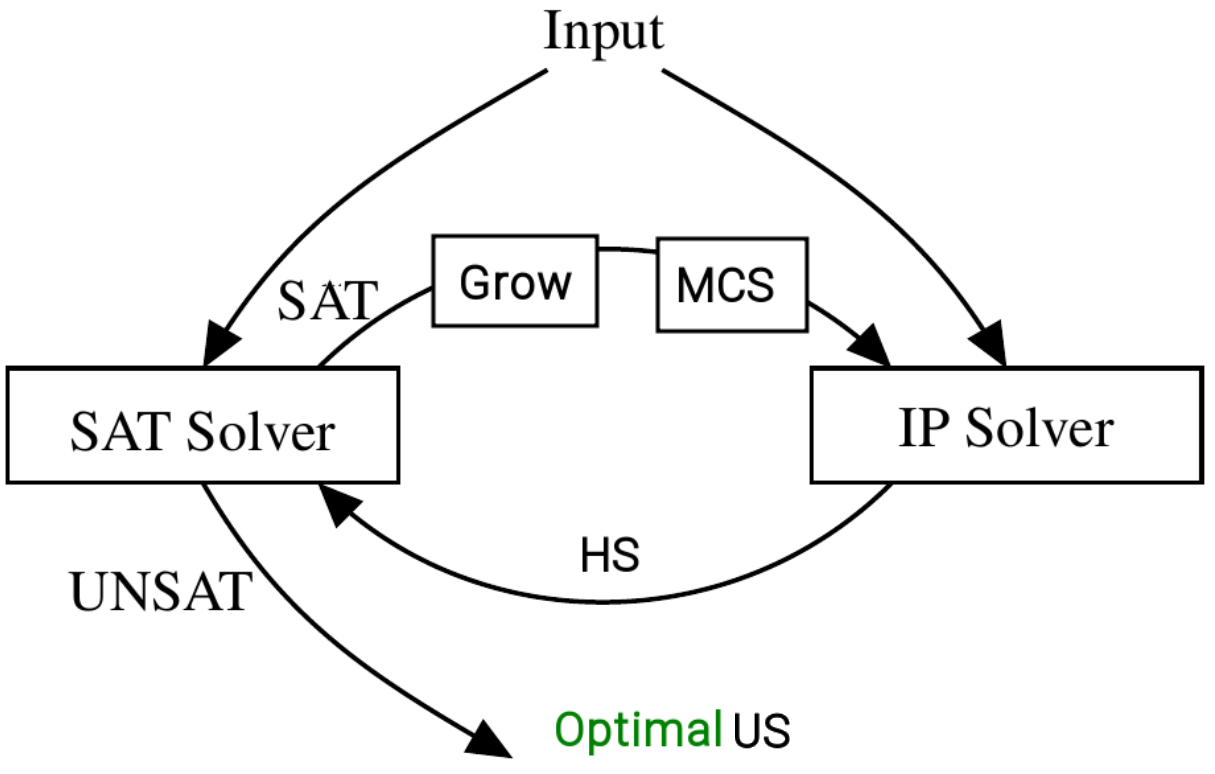
\includegraphics[width=\textwidth]{ihs.png}
%			\end{figure}
%		\end{minipage}
%	\vfill
%		\begin{figure}
%		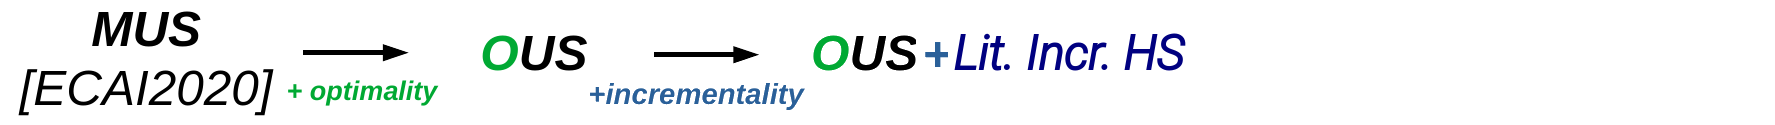
\includegraphics[width=\textwidth]{mus_to_ous_i_litincr.png}
%	\end{figure}
%	\end{frame}
%
%	\begin{frame}{Incrementality}
%	
%	\begin{minipage}{0.59\textwidth}
%		\begin{enumerate}
%			\item {\color{vuborange} Incremental \emph{OUSs}}
%			\begin{itemize}
%				\item Keep Satisfiable Subsets between OUS-calls
%				\item Naïve OUS-restart $\rightarrow$ Keep 1 MIP solver warm per literal
%				\begin{itemize}
%					\item[$\implies$] No need to keep track of Satisfiable Subsets
%				\end{itemize}
%			\end{itemize}	
%		\end{enumerate}
%	\end{minipage}
%	\begin{minipage}{0.39\textwidth}
%		\begin{figure}
%			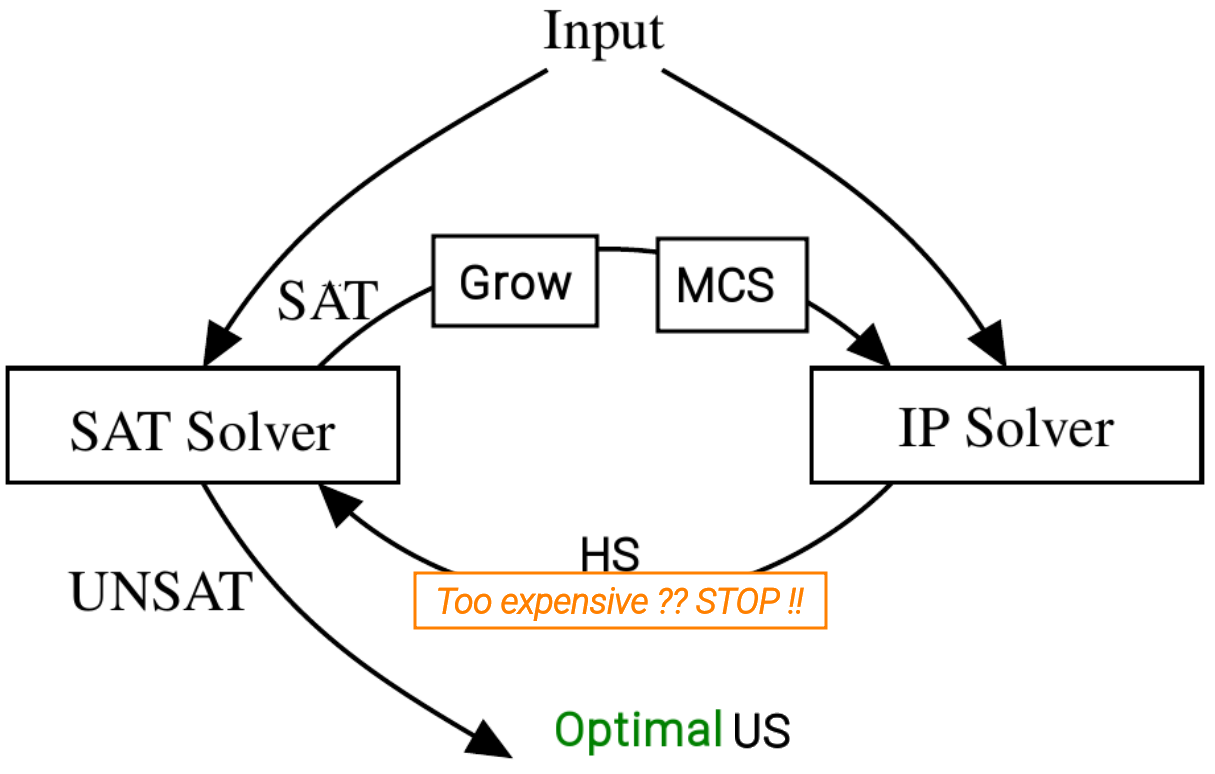
\includegraphics[width=\textwidth]{ihs_cost.png}
%		\end{figure}
%	\end{minipage}
%	\begin{enumerate}
%		\item {\color{vuborange} + Optimizations {\color{blue} (Bounded)}}
%		\begin{itemize}
%			\item Keep track of cost for computed OUSs 
%			\begin{itemize}
%				\item[$\implies$] Use previously found bound on OUS to interrupt if cost(HS) too high 
%			\end{itemize}
%			\item Sort the literals based on cost
%		\end{itemize}
%	\end{enumerate}
%	
%	\begin{figure}
%		
\includegraphics[width=\textwidth]{mus_to_ous_i_bounded.png}
%	\end{figure}
%\end{frame}
%
%\begin{frame}{Optimality \& Constrainedness}
%	\begin{figure}
%		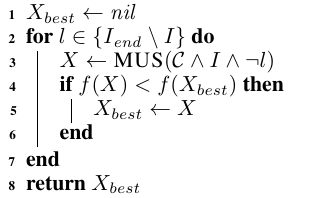
\includegraphics[width=0.45\textwidth]{algo_mus2.png}
%	\end{figure}\pause
%	{\Huge$$\downarrow$$}
%	\begin{figure}
%		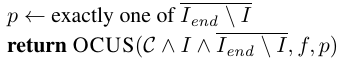
\includegraphics[width=0.5\textwidth]{exactly_one.png}
%	\end{figure}
%\end{frame}
%
%\begin{frame}{Optimality \& Constrainedness}
%	\begin{minipage}{0.49\textwidth}
%		\begin{figure}
%			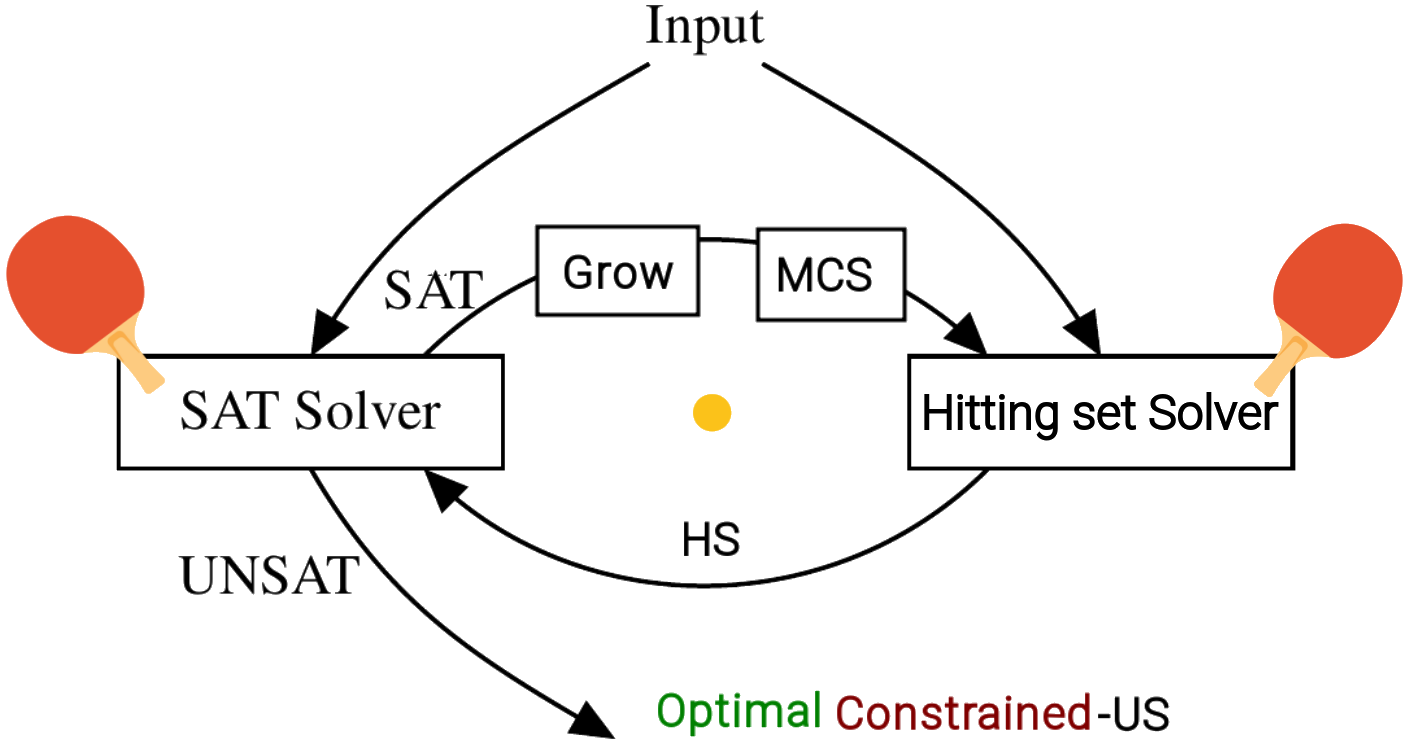
\includegraphics[width=\textwidth]{ihs_constrained.png}
%		\end{figure}
%	\end{minipage}
%	\begin{minipage}{0.5\textwidth}
%		% TODO: ADD algorithm  one step !
%		\begin{itemize}
%			\item Inspired by \cite{ignatiev2015smallest}
%			\item MIP solver instead of SAT-based
%			\item[+] Optimal Hitting set (\emph{\textbf{Optimality}})
%			\item[+] {\color{red} 1 literal explained (\emph{\textbf{Constrained}})}
%		\end{itemize}
%	\end{minipage}
%	\vfill
%	\begin{figure}[h]
%		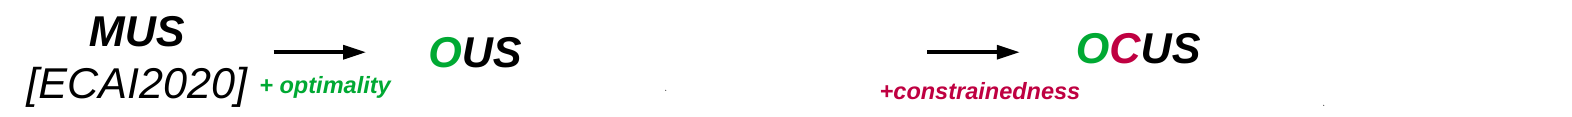
\includegraphics[width=\textwidth]{mus_to_ocus.png}
%	\end{figure}
%	
%\end{frame}
%
%\begin{frame}{Optimality \& Constrainedness + Incrementality}
%		\begin{enumerate}
%			\item \color{vuborange} Incremental \emph{OUSs} + optimizations {\color{blue} (Bounded)}\pause
%			\item {\color{vuborange} Incremental \emph{OCUS}}
%			\begin{itemize}
%				\item Naïve OCUS-restart $\rightarrow$ Keep only 1 MIP solver warm
%			\end{itemize}
%		\end{enumerate}
%		\begin{figure}
%			
\includegraphics[width=\textwidth]{mus_to_ocus_i.png}
%		\end{figure}
%	\end{frame}
%
%%\begin{frame}{Incrementality}
%%	\begin{enumerate}
%%		\item Incremental \emph{OUSs} + optimizations\pause
%%		\item {\color{vuborange} Incremnetal \emph{OCUS}}
%%		\begin{itemize}
%%			\item Naïve OCUS-restart $\rightarrow$ Keep only 1 MIP solver warm
%%		\end{itemize}
%%	\end{enumerate}
%%	\begin{figure}
%%		
\includegraphics[width=\textwidth]{mus_to_ocus_i.png}
%%	\end{figure}
%%\end{frame}
%
%\begin{frame}{Results}
%	\begin{figure}
%		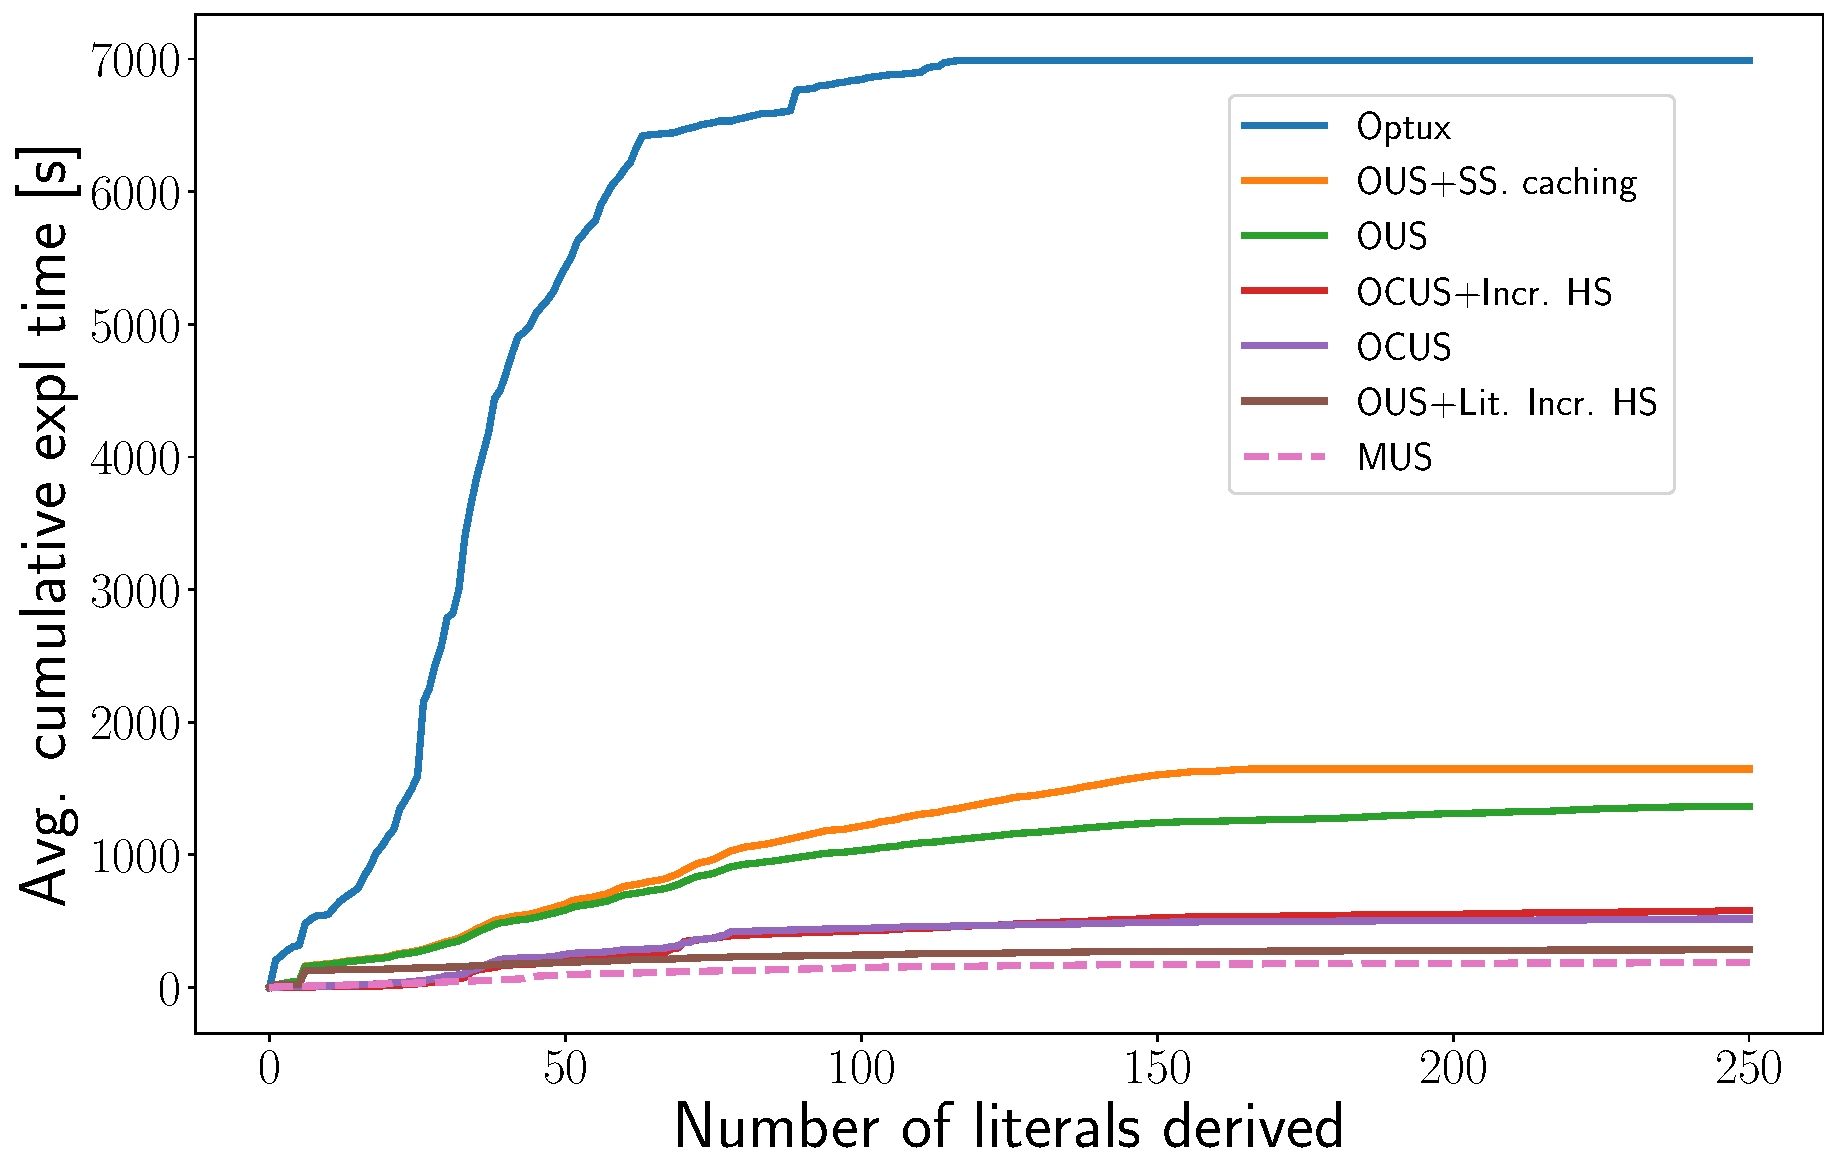
\includegraphics[width=0.9\textwidth]{figures/cumul_incr_avg_time_lits_derived_new_optux.pdf}
%	\end{figure}
%\end{frame}
%	
%	\begin{frame}{Contributions}
%		In this paper, we
%			\begin{description}[font=\color{vuborange}\itshape]
%			\item[\hspace{0.9cm}Optimality] introduce (cost-)\textbf{\underline{O}ptimal} \underline{U}nsatisfiable \underline{S}ubsets (OUS) using the minimal hitting set duality 
%			\item[\hspace{1.05cm}Efficiency] Bounded+sorted OUS calls
%			\item[Constrainedness]  analyze the structural constraints of the OUS explanations
%			\item[\hspace{0.3cm}Incrementality] improve the efficiency of explanation sequence generation
%		\end{description}
%		\vfill
%	\end{frame}
%	
%	\begin{frame}{ Vision and possibility of collaboration}
%		\framesubtitle{Improving the quality of explanation sequences}
%	\begin{description}
%		\item[Sequence-level]  Which explanations should be derived first ?
%		\begin{itemize}
%			\item Explore the relations between explanations 
%		\end{itemize}
%		\item[Sequence-level] How are the explanation sequences performing on other puzzles ? \cite{espasa2021using}
%		\begin{itemize}
%			\item Explore more logic grid puzzles
%			\item Explore other types of puzzles
%		\end{itemize}
%		\item[Explanation-level] How do we adapt the explanations based on the preferences of the user ? 		
%		\begin{itemize}
%			\item Better quality explanations 
%		\end{itemize}
%		\item[Explanation-level] Which explanation difficulty metric is best ? 
%		\begin{itemize}
%			\item Better quality explanations 
%		\end{itemize}
%	\end{description}	
%	\end{frame}
%	
	\begin{frame}[allowframebreaks]
		\frametitle{References}
		\bibliographystyle{named}
		\bibliography{refs}
	\end{frame}
%	
%	\begin{frame}{Results}
%			\begin{figure}
%			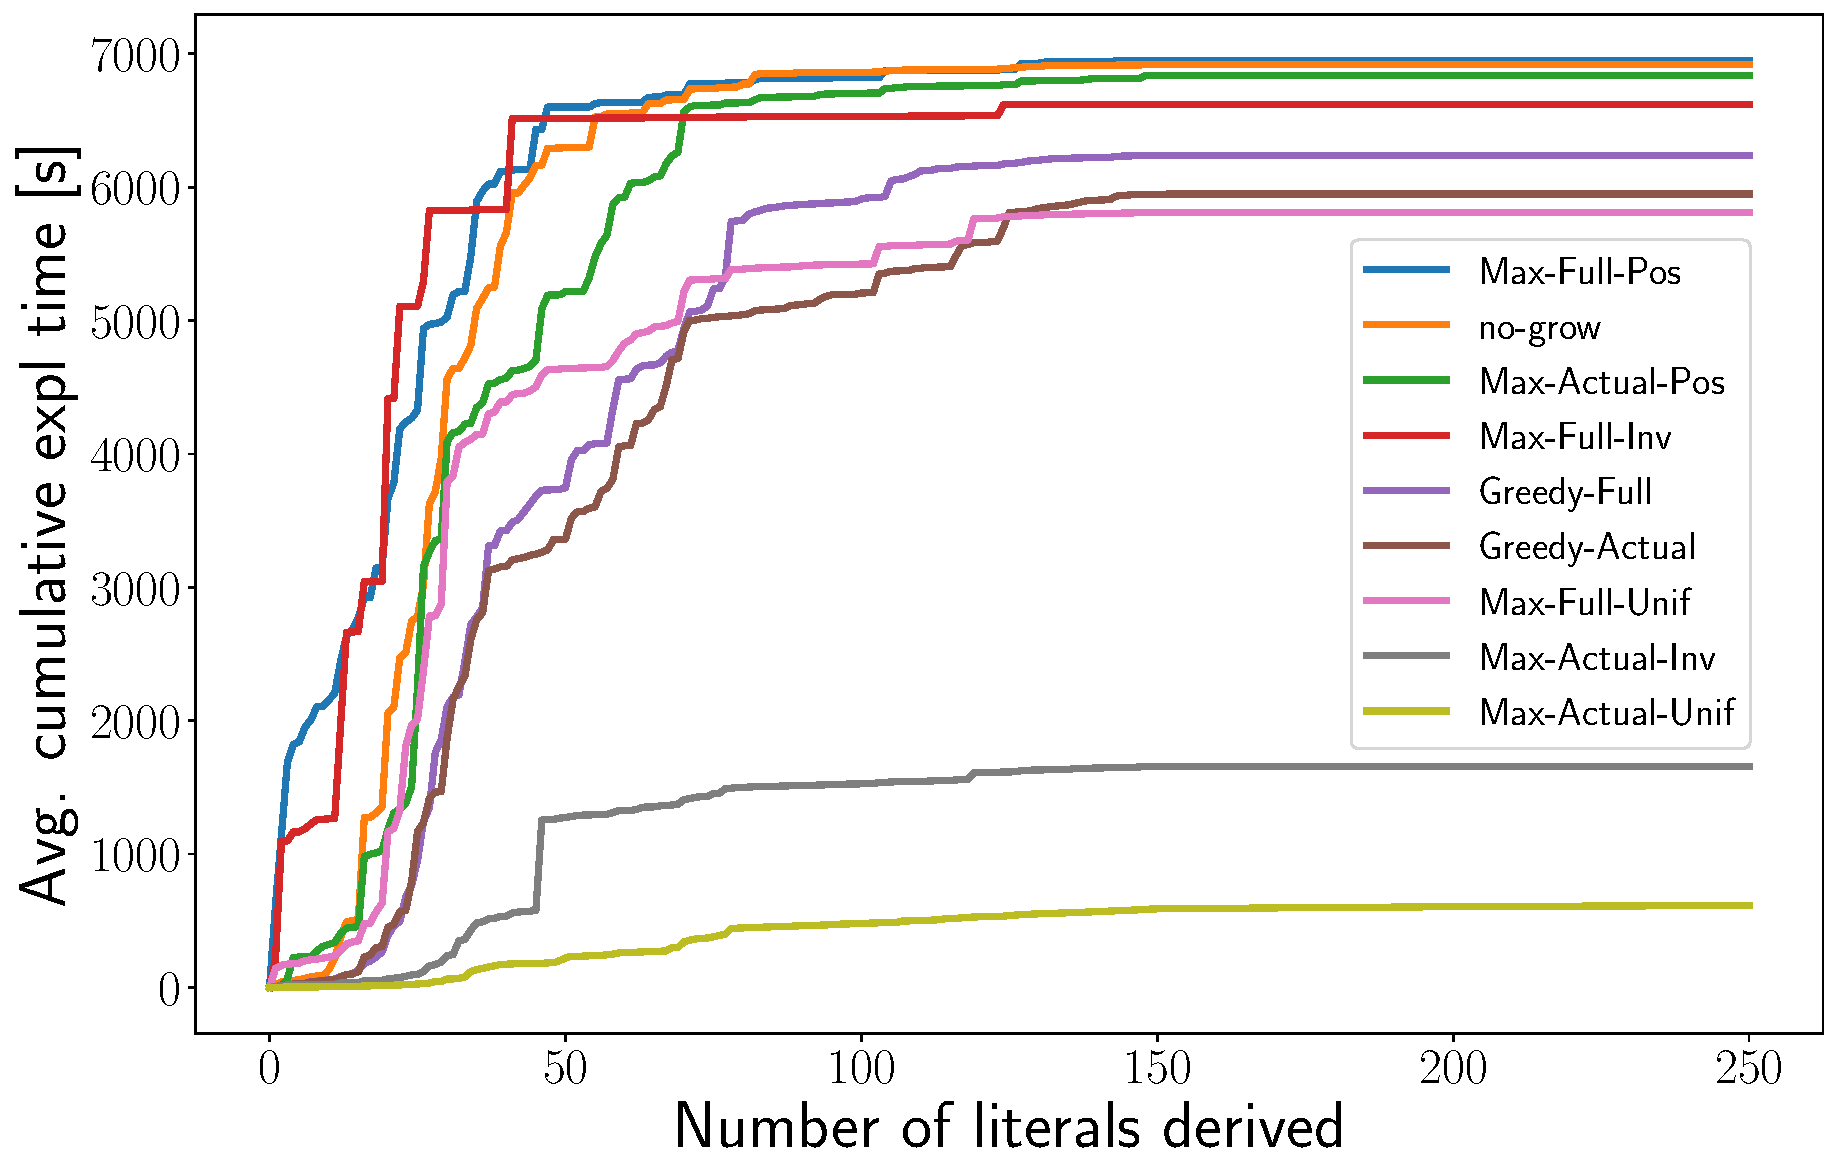
\includegraphics[width=\textwidth]{figures/new_cumul_grow_avg_time_lits_derived_new.pdf}
%		\end{figure}
%
%	\end{frame}
	
\end{document}